\documentclass[11pt]{article}

\usepackage{common}
\usepackage{booktabs}
\usepackage{wrapfig}
\usepackage{titling}
\usepackage{titlesec}
\usepackage{float}
\usepackage[margin=0.99in]{geometry}

\titlespacing\section{0pt}{4pt}{2pt}
\setlength{\parskip}{0.35em}
\setlength{\droptitle}{-5em}
\pagestyle{plain}


\title{Practical 2: Classification\\ Classifying Malicious Software}
\author{Antonio Copete, acopete@cfa.harvard.edu, Camelot.ai Copete \\
	Fangli Geng, fgeng@g.harvard.edu, Camelot.ai fangligeng\\
	Junran Yang, jyang3@gsd.harvard.edu, Camelot.ai junran}

\begin{document}
\maketitle{}

%\citep{canali} 
%\citep{canzanese}
%\citep{rozenberg}

\section{Technical Approach}

The purpose of this practical was to classify a test set of 3,724 files in XML format into 15 classes of malware, using a training set of 3,086 labeled files. Our general approach consisted on the following steps:

\begin{enumerate}
\item \textbf{Feature Engineering}\\
Initial inspection showed the XML data files to be structured hierarchically into a series of \emph{processes}, in turn composed of a series of \emph{threads}, in turn composed of a series of \emph{system calls}. Each of these were identified by a \emph{tag} as well as a number of \emph{attributes} indicated as sets of key-value pairs. Our simplest approach began by drawing $n$-grams (ordered sets) of up to 4 consecutive system call tags, initially without attributes, and our initial exploratory analysis tested the hypothesis that the presence and order of such system call tags was correlated with the distinct anomalous behavior found in different types of malware.

More advanced versions of this approach found in the literature (REF: Canali et al) suggested also drawing features based of $n$-bags (unordered non-consecutive sets) as well as $n$-tuples (ordered non-consecutive sets) of system calls and processes, as well as including attributes such as file names, file sizes, URLs, execution times, etc. We found some of these attributes to be predictive of some specific classes, such as the file \verb|maxtrox.txt| being always related to malware of class VB, and \verb|GrayPigeon_Hacker.com.cn| always indicating malware of class Hupigon. In addition, we also took into account the number of total processes and thread numbers.

To analyze the system call tags (including 4-grams, 29,813 features in total) and suspicious attributes (110,465 features in total), we tried 2 methods: using either the number of counts, or the TF-IDF (term frequency---inverse document frequency) [REF: System Call-based Detection of Malicious Processes.pdf]. The TF-IDF value measures the relative frequency of a token across the data set; it is proportional to the number of times a token appears in a given file, offset by the frequency of the token across all files, which helps adjust for the absolute frequency of a given token in the whole dataset. The scikit-learn module \verb|sklearn.feature_extraction.text| includes the objects \verb|CountVectorizer| and \verb|TfidfVectorizer|, which tokenize large strings of tags (with or without arguments) into $n$-grams, and then transform them into counts and TF-IDF values in the resulting feature matrix, respectively.


\item \textbf{Feature Selection}\\
Since we derived roughly 140,000 features from a training set of just over 3,000 files, it was easy to cause our model to overfit the data. To avoid overfitting, we used the sklearn module \verb|SelectFromModel| and the classifier \verb|sklearn.ensemble.RandomForestClassifier| to reduce features and use cross-validation to determine the features we want to keep. More specifically, we ran a loop to continuously drop features with importance of less than 10\% the mean importance across all features, monitoring the mean score from 5-fold cross-validation in each iteration. The highest score happened with around 5,000 features, which was 1/20 of the original feature size.
% Antonio: I also dropped features with low variance across both the training and test set (unsupervised feature selection), and used a similar strategy to drop features according to RF importance. I went more conservatively and dropped only features that had importance = 0 in all 5 cross-validation sets. But Fangli's strategy is good, so we can leave it at that.

\item\textbf{Model Selection}\\
We began by exploring a number of classifiers for model selection from scikit-learn, including \verb|RandomForestClassifier| (Random Forest), \verb|svm.SVC| and \verb|svm.LinearSVC| (Support Vector Machine), and \verb|linear\_model.SGDClassifier| (Stochastic Gradient Descent), with default hyper-parameters. The Random Forest classifier yielded the best score of 0.78105 on the test data, compared to 0.57211 for SVC, 0.76789 for Linear SVC, and 0.77158 for SGD. We thus selected Random Forest as our main model and proceeded to tune it in the subsequent steps.

In addition, we found the class distribution in the training set to be heavily imbalanced. We therefore took a sequential approach to model training, dividing the data into 4 main categories: None (52.14\%), Swizzor (17.56\%), VB (12.18\%) and Others (18.12\%). We first trained the model on each of first 3 categories, and then separately on the minor categories. This approach resulted in an improvement of 0.02 in the test score, compared to training on all categories jointly (0.81211 vs 0.79263). We tried the same approach on a Neural Network for comparison, yielding a score of 0.79105 for training on separate categories, and confirming again Random Forest as the better model.

Late in the process we also found a bug in the original code we were provided for extracting system call tags, which was causing the tags for every other thread to be skipped altogether. Our final results are based on the corrected version of feature extraction, but due to time constraints we limited ourselves to 4-gram tokens of system call tags without attributes. With the corrected feature set and a Random Forest classifier trained jointly across all categories, we obtained an improvement of 0.015 in the test data score (0.80789 vs 0.79263).

In our last attempt at model experimentation, we were inspired by a Microsoft Malware Classification Challenge (BIG2015)\footnote{https://www.kaggle.com/c/malware-classification/discussion/13897} to utilize xgboost and a semi-supervised method to detect malware from assembly code. Gradient Boosting is different from Random Forest in that it focuses more on reducing the bias rather than variance. After grid searching for hyperparameters, the highest accuracy we got by xgboost was 0.82526. Furthermore, we tried semi-supervised Gradient Boosting, aiming to further reduce the bias of the model and incorporating information from test dataset into training dataset. We first generate pseudo labels for the test set by choosing the maximum probability of our best model. Then we predict on the test set again in a cross-validation fashion with both training data and test data.

For example, the test data set is split to 4 parts: A, B, C and D. We use the entire training data, and test data A, B, C with their pseudo labels together as the new training set, and we predict on test set D. The same method is used to predict on A, B and C. However, this approach didn't provide us with decent results. We suspect the relatively low accuracy in the prediction set (0.82526) provided more inaccurate information than that it could offer to reduce bias.

 
\end{enumerate}


\section{Results}

\begin{table}
\centering
\begin{tabular}{cccccccc}
 \toprule
 Rank & max\_depth & eta & min\_child\_weight & colsample & cv mean error & best num\_round & final score\\
 \midrule
  1 & 4 & 0.15 & 1 & 0.5 & 0.0933316 & 49 & 0.82158\\
  2 & 6 & 0.2 & 1 & 1 & 0.093334 & 25 & 0.811054\\
  3 & 4 & 0.1 & 1 & 0.5 & 0.093983 & 68 & 0.82526\\
  4 & 4 & 0.15 & 2 & 0.5 & 0.094306 & 54 & - - -\\
  5 & 6 & 0.15 & 1 & 1 & 0.0949526 & 31 & - - -\\
 \bottomrule
\end{tabular}
\caption{\label{tab:results} Result tables for the best 5 cross-validation scores by Gradient Boosting with grid search}
\end{table}

Table 2 shows the best 5 cross-validation scores by Gradient Boosting with grid search. The hyper-parameters we tuned were max\_depth (the maximum depth of a tree, same as GBM, set as 2, 4, 6), eta (analogous to learning rate in GBM, set as 0.05, 0.1, 0.15, 0.2),  min\_child\_weight (defines the minimum sum of weights of all observations required in a child, set as 1, 2), colsample\_bytree (denotes the subsample ratio of columns for each split, in each level, set as 0.5, 1). Those 48 configurations were selection based on what we found people commonly used. We also tested models with higher and lower rounds numbers, which were different from what were the best indicated by cross-validation. Then we found it would give us worse performance by using those round numbers, compared to that from best round numbers setting given by cross validation.


\begin{figure}[H]
\minipage{0.5\textwidth}
  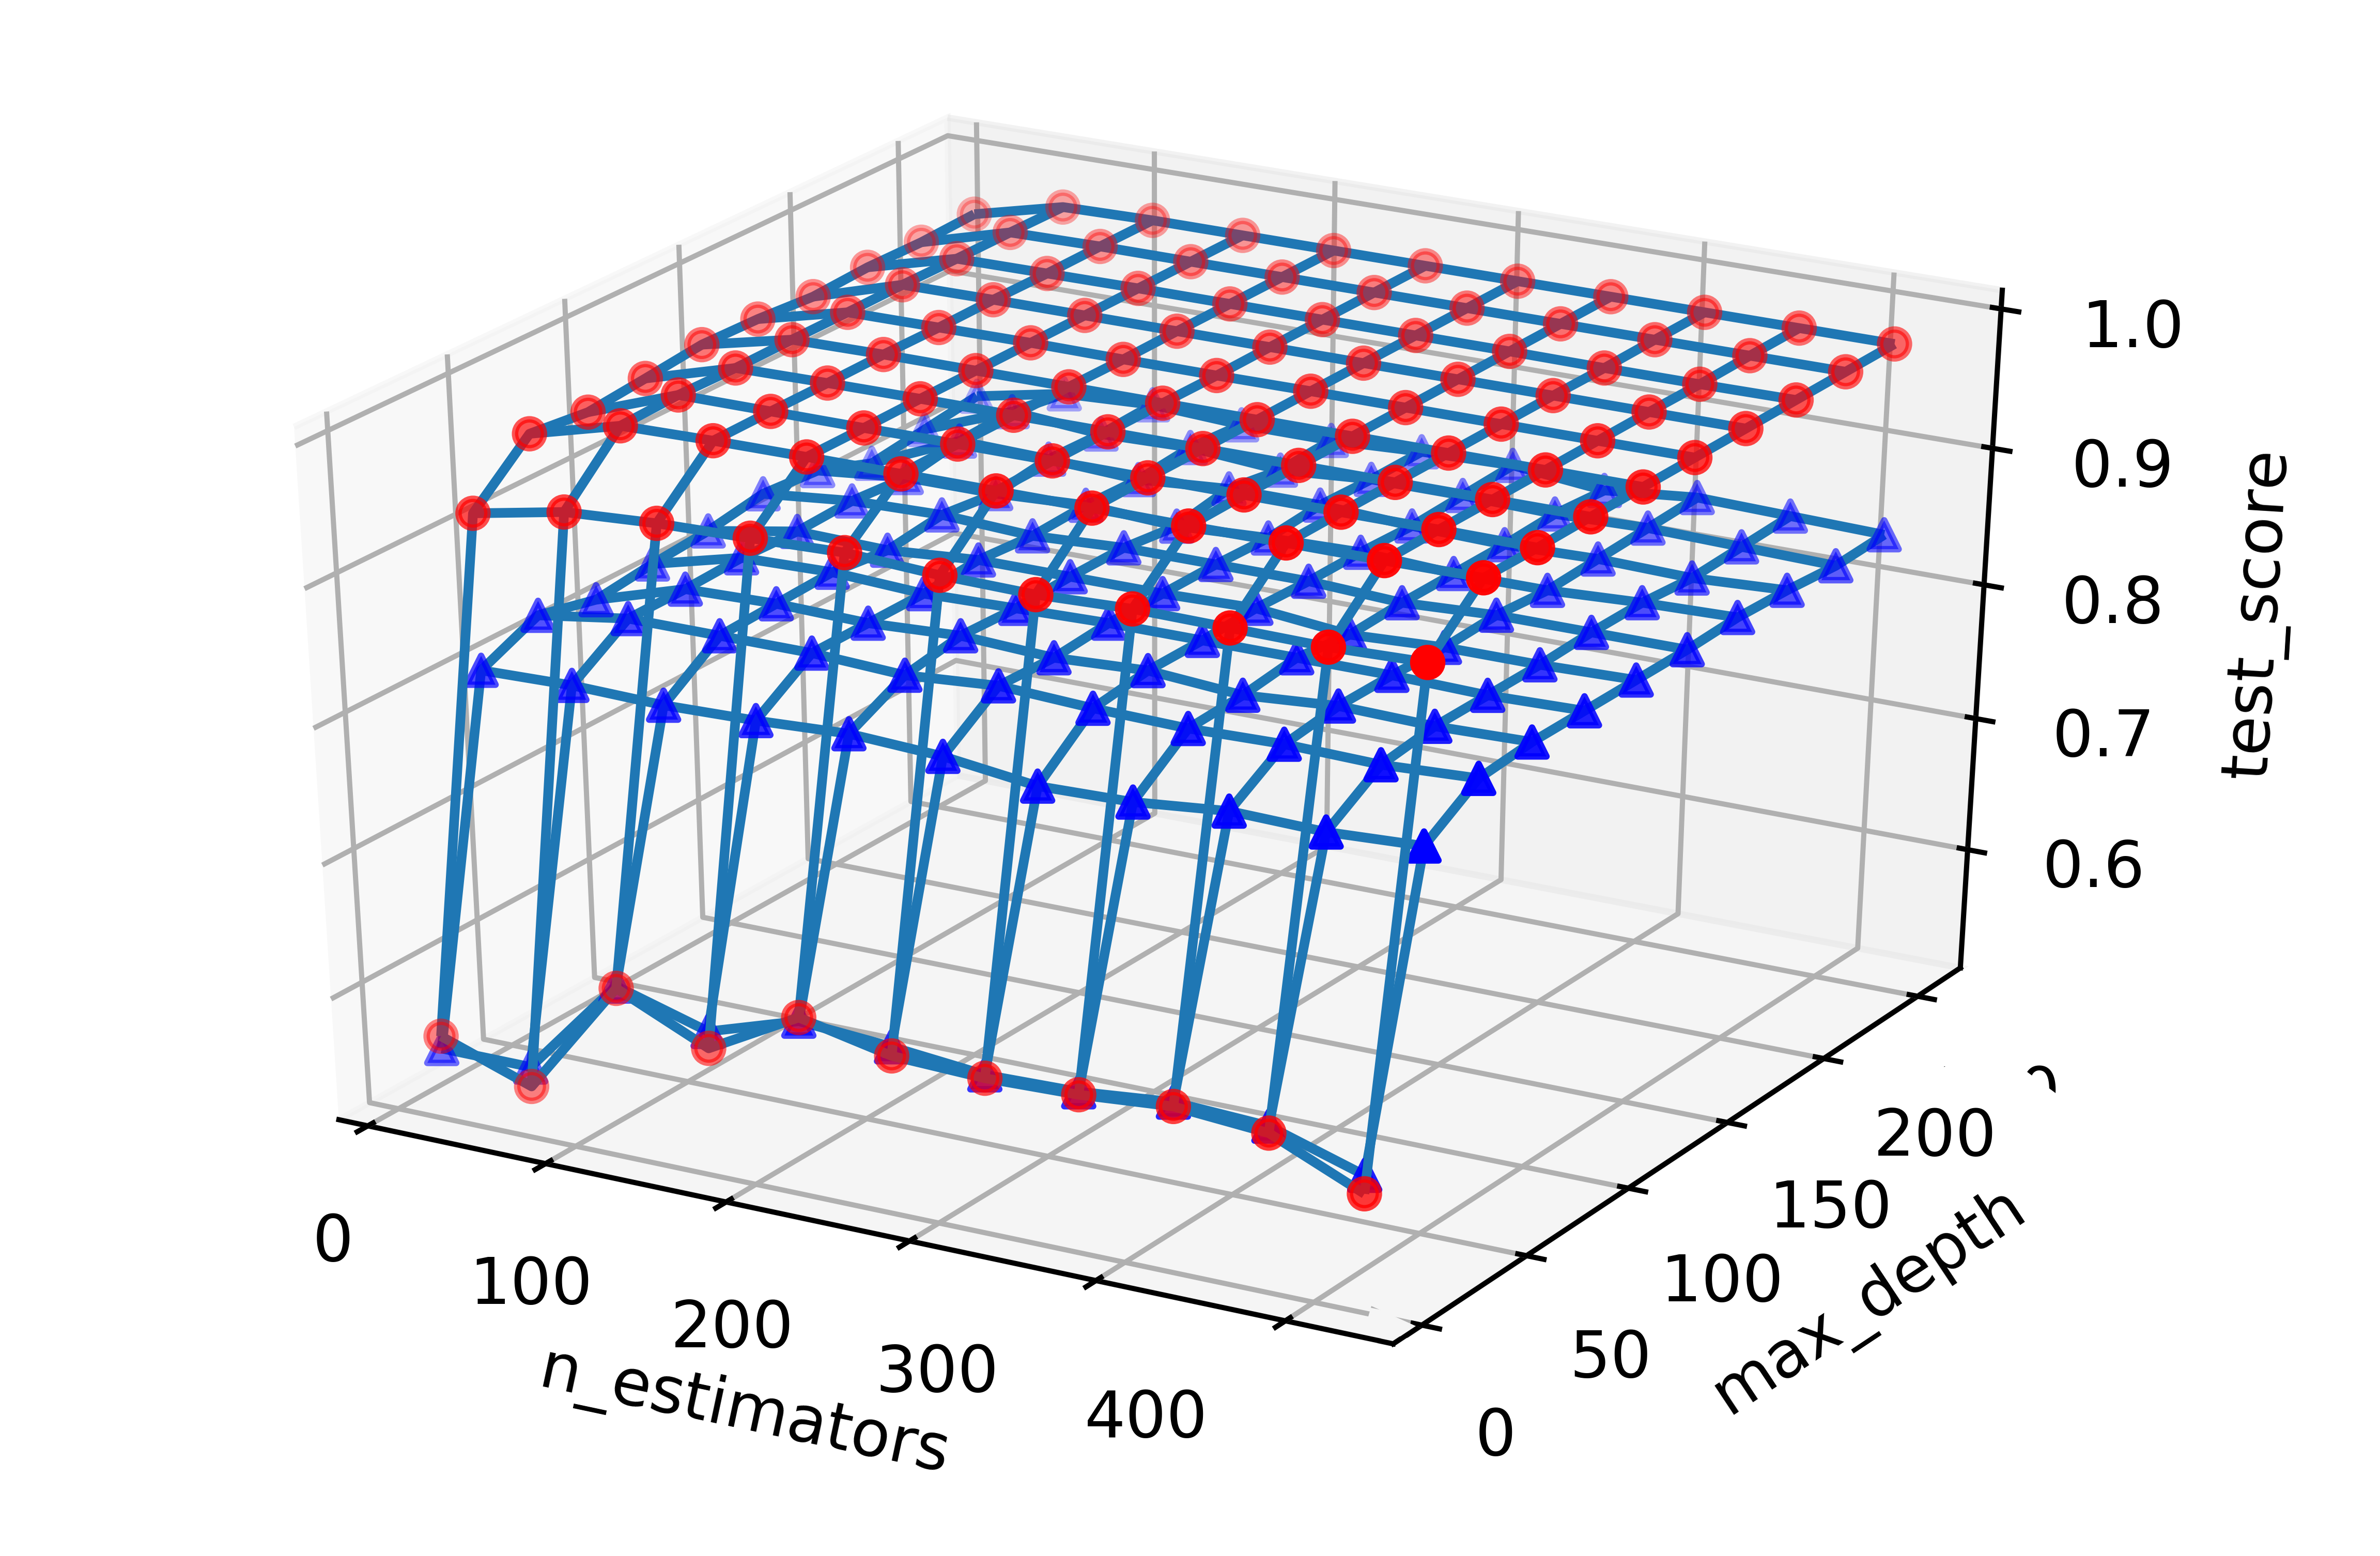
\includegraphics[width=\linewidth]{hyperparameter_tuning_1}
  \caption{Max depth range from 10 to 235, and number of estimators range from 10 to 460.}
  \label{fig:results}
\endminipage\hfill
\minipage{0.5\textwidth}
  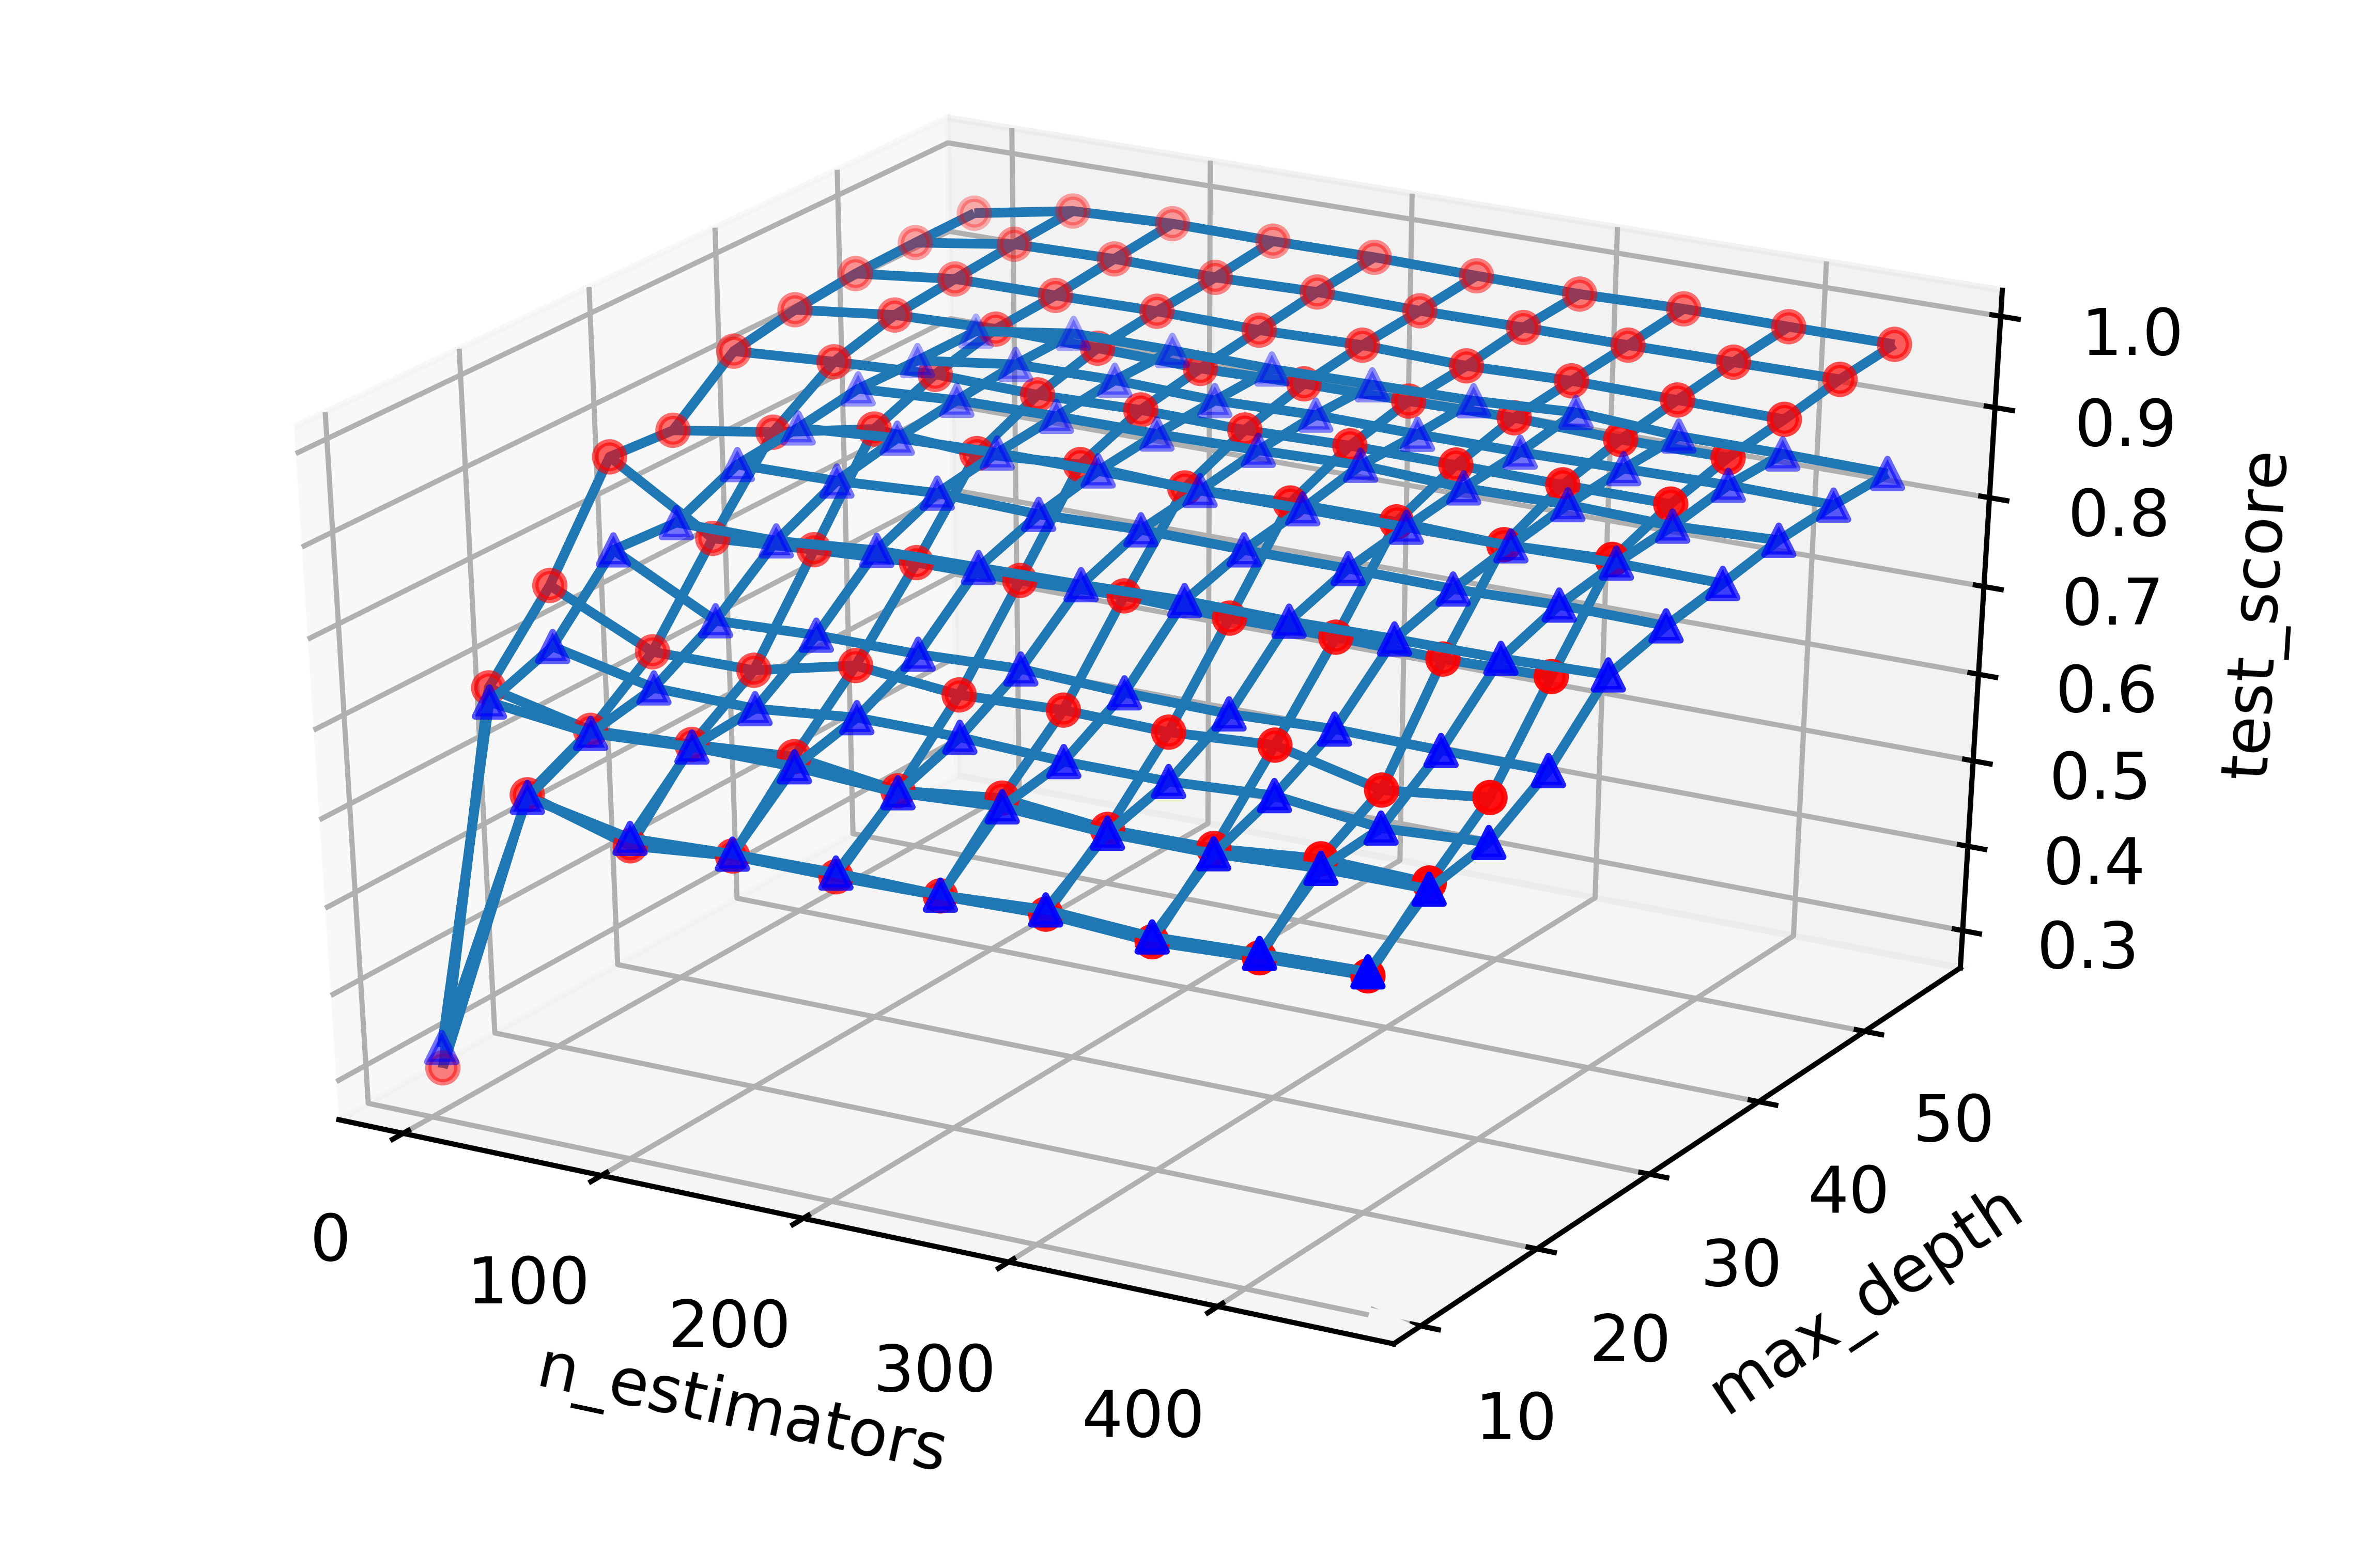
\includegraphics[width=\linewidth]{hyperparameter_tuning_2}
  \caption{Max depth range from 10 to 45, and number of estimators range from 10 to 460.}
  \label{fig:results}
\endminipage\hfill
\minipage{1\textwidth}
  \begin{center}
  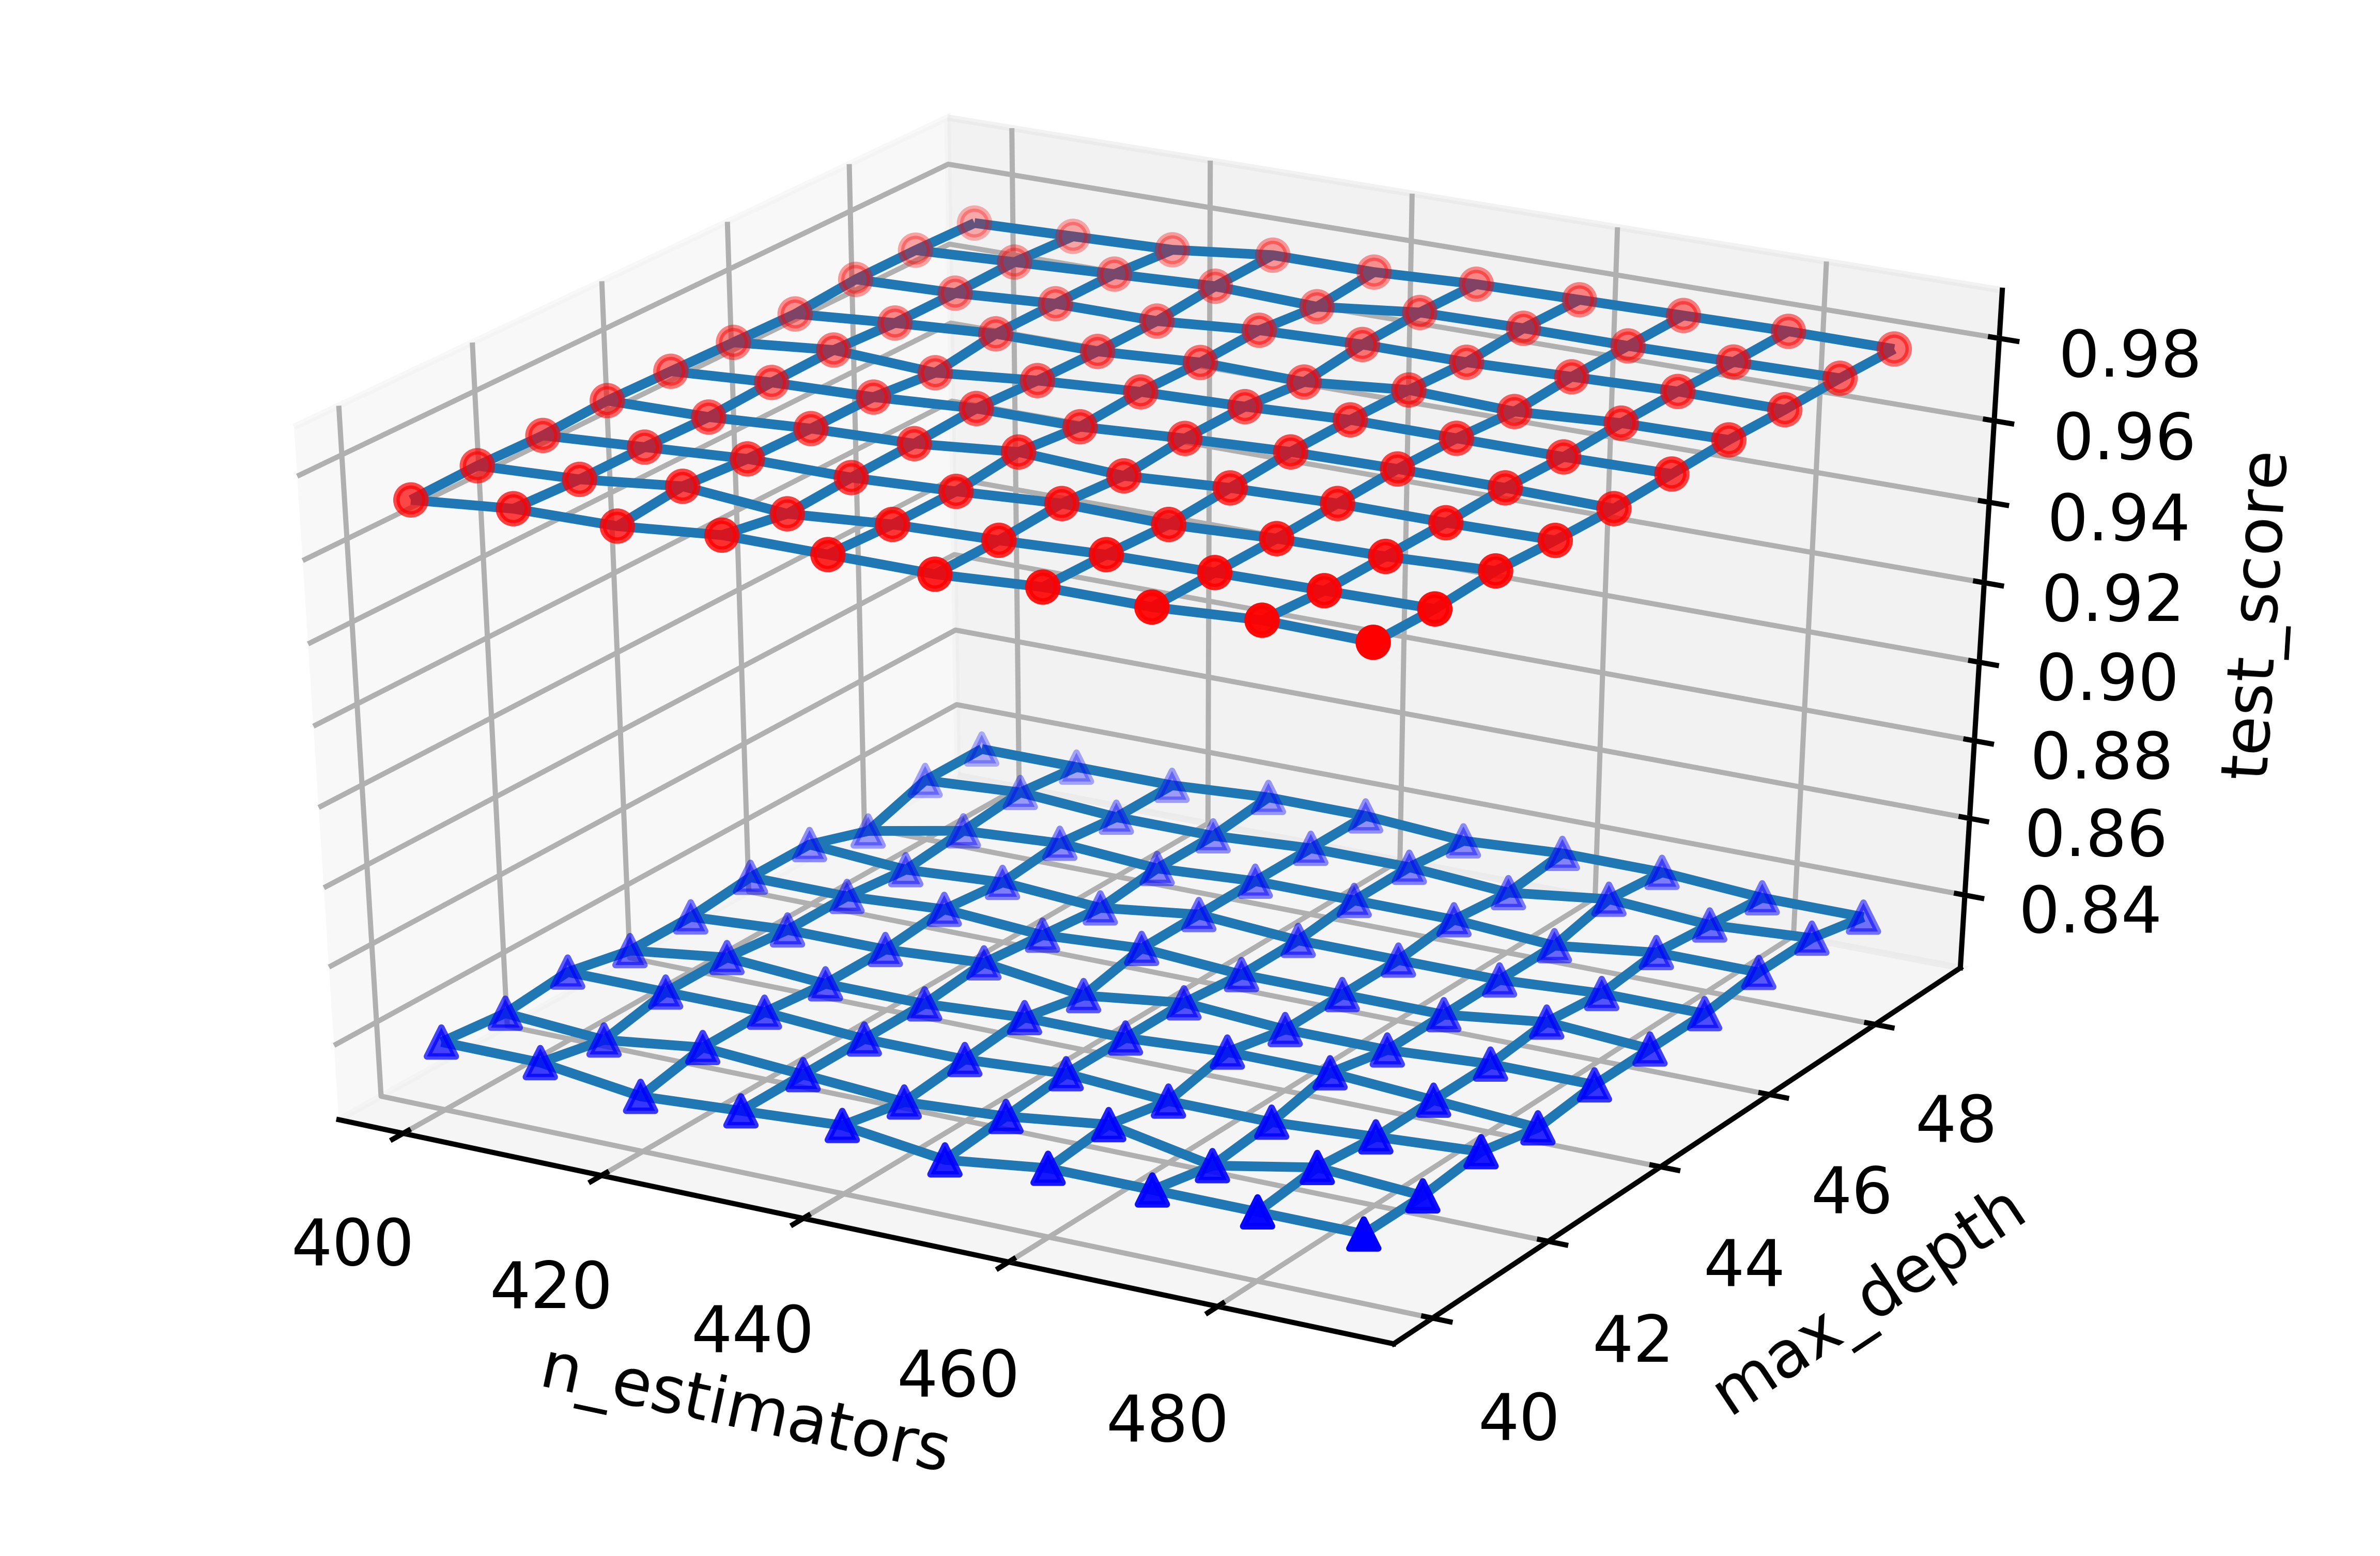
\includegraphics[width=0.5\linewidth]{hyperparameter_tuning_3}
  \caption{Max depth range from 40 to 49, and number of estimators range from 400 to 490.}
  \label{fig:results}
  \end{center}
\endminipage
\end{figure}

Figure 1-3 show the hyper parameter tuning process for random forest model. We first ran the experiment in a rough region: max\_depth range from 10 to 235 with a step of 25, while n\_estimators range from 10 to 460 with a step of 50. From this experiment we found out that when depth is larger than 60, the increasing depth of the decision tree no longer contributes to train score or test score. That is because we only have a training set of around 3000 samples, and making the tree deeper than the square root of number of samples could not contribute to the accuracy of the decision trees. \\
Then we ran 2 experiments with finer sampling. We found out from the results that we should make the depth as close to the square root of number of samples as possible, while choosing number of estimators to be around 400, since larger number of estimators no longer improve the performance of the model significantly. 

\section{Discussion} 

First, we focused on new feature generating process. We came up with 1-gram, 2-gram, 3-gram, 4-gram, 10-gram of system call tags, useful system call attributes we identified, TFIDF for feature scaling. Then, based on the classification task we were give and the limited sample size we faced, we decided to test several different basic models (Random Forest Classifier, C-Support Vector Classifier, Linear-Support Vector Classifier, Stochastic Gradient Decent classifier) with different subsets of those data. With the results from those experiments, we decided to narrow down to Random Forest and deeply tune the hyperparameters to achieve best possible results. We further improved the Random Forest approach by 2-step classification, in order to capture more detail information in the Malware categories with low percentage. As the results is still not ideal with a 0.816 accuracy score, we did The accuracy can be higher with full feature scaled by TF-IDF. Furthermore, aiming to reduce the bias of the overfitting models, we took Gradient Boosting approach, which ended up giving the best accuracy among all the models we tested. 

If there were more time to pursue better estimates, we would try to resample from the original data set as new training sets to reduce bias, and further tune semi-supervised Gradient boosting models. We also consider to create a 2-step Gradient Boosting approach to capture more detail information in the small malware categories as what we did for Random Forest.

\bibliography{P2_dualspace}

\end{document}

